\section{Detector Simulations}

Detailed simulations of the FT have been done with the Geant4-based Monte Carlo code for CLAS12,
GEMC~\cite{gemc} to optimize the detector design, to develop the reconstruction algorithms, and to understand
the detector performance.

Details on the implementation in GEMC of the detector geometry and digitization are reported in Ref.~\cite{gemc},
while an extensive discussion of the simulation studies that guided the detector design are presented in
Ref.~\cite{ft-tdr}. Here we focus on summarizing the results of the simulation studies that are relevant to
understand the FT performance.

\subsection{Leakage Corrections}

The reconstructed cluster energy can be systematically smaller than the actual energy of the particle that
induced the shower due to leakages in the shower containment caused by the limited dimensions of the
calorimeter, by cuts in the clustering algorithms, and thresholds in the hit detection. An example of the difference
between the reconstructed cluster energy and the simulated electron energy is shown in the top panel of
Fig.~\ref{fig:gemc_leakage}. This was obtained assuming an equivalent threshold on  the individual crystals of
10~MeV: the leakage varies from $\sim$80~MeV (16\%) for 500~MeV electrons to $\sim$300~MeV (6.6\%) for
4.5~GeV electrons.

This effect can be easily corrected for by parameterizing the leakage as a function of the reconstructed cluster
energy and position, and applying the correction in reconstruction. Simulations of single electrons were performed
in GEMC and the difference between the reconstructed cluster energy and the electron energy was studied as a
function of the cluster seed crystal. For each crystal, the dependence of this difference on the reconstructed
cluster energy was fitted to a fourth-order polynomial function, which was then used as an additive correction to
the reconstructed cluster energy. The final dependence of the difference between corrected cluster energy and
simulated energy is shown in the bottom panel of Fig.~\ref{fig:gemc_leakage}.

\begin{figure}
\includegraphics[height=\columnwidth]{fig/gemc_leakage.eps}
\caption{Top: difference between the simulated electron energy and the reconstructed cluster energy as a function
  of the electron energy for a 10~MeV equivalent threshold on the single crystal signal. Bottom: difference between
  the simulated electron energy and the cluster energy after the leakage correction.}
\label{fig:gemc_leakage}
\end{figure}

\subsubsection{Electromagnetic Background and Radiation Dose}

The electromagnetic background produced by the interaction of the electron beam in the target  at the nominal
CLAS12 luminosity was simulated in GEMC. For this purpose, in each event, about 124k, 11~GeV electrons were
generated that originated 10~cm upstream the target. The electrons were distributed randomly with the
radio-frequency structure of the beam in a 250~ns window. This number of electrons corresponds to the number
of beam electrons that would pass through the target in the chosen time window at the nominal CLAS12 luminosity
of 10$^{35}$~cm$^{-2}$s$^{-1}$. These simulations were used to study background rates in each of the FT detectors,
to determine the pile-up probability, and to estimate the radiation dose the FT would be subject to during operations.

The overall particle rate in the FT was found to be about 120~MHz, dominated by very low energy particles and with
only 6\% due to particles with energy above 100~MeV. In the energy range to be tagged (0.5-4.5~GeV) the overall
particle rate is further reduced to about 180~kHz, equally shared between photons and hadrons. 

For the FT-Cal, the energy deposition in each crystal was evaluated from the background simulation and used to
calculate the dose per unit of time. The overall radiation dose at $10^{35}$~cm$^{-2}$s$^{-1}$ was estimated to be
less than 1.5~rad/hr when averaged over the entire calorimeter with a distribution on the calorimeter crystals as
shown by Fig.~\ref{fig:ft_rad}. The maximum dose per crystal is of about 3~rad/hr, which would result in an
maximum integrated dose per crystal of about 2160~rad in 30~days of beam time.

\begin{figure}
\includegraphics[height=0.9\columnwidth]{fig/ft_rad.eps}
\caption{Radiation dose on the FT calorimeter crystals in rad/hour at $10^{35}$~cm$^{-2}$s$^{-1}$ luminosity. The
  maximum values of about 5~rad/hr are observed for the innermost crystals, i.e. at the smaller angles.}
\label{fig:ft_rad}
\end{figure}
